\documentclass[12pt]{article}
\usepackage{graphicx}
\usepackage{titlesec}
\usepackage{fancyhdr}
\usepackage{listings}
\usepackage{xcolor}
\usepackage{hyperref}
\usepackage{caption}
\usepackage{subcaption}
\usepackage{geometry}
\usepackage{tikz}
\geometry{margin=1in}
\pagestyle{fancy}
\fancyhf{}
\rhead{GENAI Project Report}
\lhead{IBM}
\rfoot{Page \thepage}

\definecolor{codebg}{rgb}{0.95,0.95,0.95}
\lstset{
  backgroundcolor=\color{codebg},
  basicstyle=\ttfamily\small,
  frame=single,
  breaklines=true,
  language=Python,
  keywordstyle=\color{blue},
  commentstyle=\color{gray},
  stringstyle=\color{green!50!black}
}

\titleformat{\section}{\Large\bfseries}{\thesection}{1em}{}

\begin{document}

% 1ST PAGE - TITLE PAGE
\begin{titlepage}
    \centering
    
\includegraphics[width=3cm]{college_logo}\hfill
    
\includegraphics[width=3cm]{ibm_logo}
    \vfill
    {\Huge\bfseries Course-Recommendation-Bot\par}
    \vspace{1cm}
    {\Large Taticherla Gnana Sai Siddartha\par}
    {\large Roll Number: 22BCE8086\par}
    \vspace{0.5cm}
    {\large VIT-AP\par}
    {\large Branch: CSE- AI\&ML\par}
    \vspace{1.5cm}
    {\large\itshape Date of Submission: \today\par}
    \vfill
\end{titlepage}

% 2ND PAGE - TABLE OF CONTENTS
\tableofcontents
\newpage

% 3RD PAGE - INTRODUCTION, OBJECTIVE, TOOLS
\section{Introduction}
A course recommendation bot to help out my fellow students. 
\newline
\newline
There are a bunch of confused individuals out there, who are interested to use their time productively by learning new courses and earning certificates, but often gets confused on what needs to be done. Here comes the chat-bot of mine for the rescue.
\newline
\newline 
IBM Watsonx and the course recommendation chatbot enable the following:

\begin{itemize}
    \item Uses IBM Watsonx and retrieval-augmented generation (RAG) to offer personalized course recommendations based on individual interests, background, and current skill level.
    \item Helps students find relevant certification options and learning materials through IBM's AI capabilities.
    \item Dynamically pulls information from a curated course database using IBM Watsonx to clarify choices.
    \item Allows students to make informed decisions about improving their skills without feeling overwhelmed.
    \item Integrates into an easy-to-use web interface powered by IBM Watsonx for natural, interactive conversations.
    \item Offers clear guidance for students looking to explore new learning opportunities with IBM's AI assistance.
    \item Aids in tracking potential learning paths that match personal career goals.
    \item Makes the upskilling process accessible, efficient, and motivating for learners through IBM's AI infrastructure.
    \item Supports students in using their time wisely while working towards certification goals.
\end{itemize}

\section{Objective}
This project aims to give a well informed course recommendations for the users based on the prompt they provide.

\section{Tools \& Technologies Used}
\begin{itemize}
  \item IDEs: Neovim, Jupyter Notebook
  \item Libraries: Transformers, pandas, numpy, langchain, langchain\_ibm, ibm\_watsonx\_ai
  \item Platform: IBM Cloud, Python 3.10
\end{itemize}

\newpage

% 4TH PAGE - METHODOLOGY
\section{Methodology / Working}
Here’s a step-by-step explanation of the working:

\begin{itemize}
  \item Step 1: I have used a text dataset for the project to implement RAG (Retrieval Augmented Generation) and imported the dataset directly inside the IBM Watsonx.ai project as an asset.
  
  \item Step 2: Performed \textbf{tokenization and text splitting} on the dataset to prepare it for retrieval. The dataset was split into manageable chunks using character-based splitting for efficient vectorization and retrieval during the RAG process.
  
  \item Step 3: Used embeddings with the dataset chunks and employed a \textbf{foundation model} from IBM Watsonx.ai to generate grounded answers to user queries based on retrieved relevant chunks, forming the retrieval-augmented generation pipeline.
  
  \item Step 4: Evaluation and Deployment
\end{itemize}


\vspace{1cm}
% Optional flowchart
\begin{center}
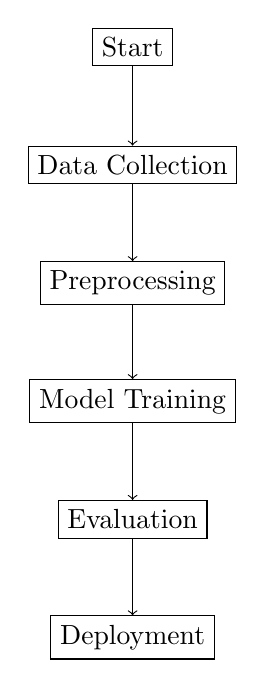
\begin{tikzpicture}[node distance=1.5cm]
  \node (start) [rectangle, draw] {Start};
  \node (data) [rectangle, draw, below of=start] {Data Collection};
  \node (prep) [rectangle, draw, below of=data] {Preprocessing};
  \node (train) [rectangle, draw, below of=prep] {Model Training};
  \node (eval) [rectangle, draw, below of=train] {Evaluation};
  \node (end) [rectangle, draw, below of=eval] {Deployment};
  \draw[->] (start) -- (data);
  \draw[->] (data) -- (prep);
  \draw[->] (prep) -- (train);
  \draw[->] (train) -- (eval);
  \draw[->] (eval) -- (end);
\end{tikzpicture}
\end{center}

\newpage

% 5TH TO 8TH PAGES - CODE SNIPPETS
\section{Code Snippets with Explanation}

\subsection*{1. Importing the Model}
\begin{lstlisting}
from ibm_watsonx_ai.foundation_models.utils.enums import ModelTypes
model_id = ModelTypes.GRANITE_13B_INSTRUCT_V2
\end{lstlisting}

\subsection*{2. Installing Dependencies}
\begin{lstlisting}
!pip install "langchain-core==0.1.24" | tail -n 1 
!pip install "ibm-watsonx-ai>=0.2.6" | tail -n 1
!pip install -U langchain_ibm | tail -n 1
!pip install wget | tail -n 1
!pip install sentence-transformers | tail -n 1
!pip install "chromadb==0.3.26" | tail -n 1
!pip install "pydantic==2.7.1" | tail -n 1
!pip install "sqlalchemy==2.0.1" | tail -n 1
\end{lstlisting}

\subsection*{3. Getting Credentials}
\begin{lstlisting}
import os, getpass
credentials = {
    "url": "https://us-south.ml.cloud.ibm.com",
    "apikey": getpass.getpass("Please enter your WML api key (hit enter): ")
}
\end{lstlisting}

\subsection*{4. Obtaining Project ID}
\begin{lstlisting}
try:
    project_id = os.environ["PROJECT_ID"]
except KeyError:
    project_id = input("Please enter your project_id (hit enter): ")
\end{lstlisting}

\subsection*{5. Fetching Dataset from IBM COS}
\begin{lstlisting}
import os, types
import pandas as pd
from botocore.client import Config
import ibm_boto3

cos_client = ibm_boto3.client(service_name='s3',
    ibm_api_key_id='wO1xV2-E45hGTkCtdLdLi6T7UuZGS3Ii2hyLrjjWsBcU',
    ibm_auth_endpoint="https://iam.cloud.ibm.com/identity/token",
    config=Config(signature_version='oauth'),
    endpoint_url='https://s3.direct.us-south.cloud-object-storage.appdomain.cloud')

bucket = 'foxofwisdom-donotdelete-pr-qyfzkqdje9z8q0'
object_key = 'sample_learning_paths.txt'

streaming_body_0 = cos_client.get_object(Bucket=bucket, Key=object_key)['Body']
\end{lstlisting}

\subsection*{6. Creating a File for the Dataset}
\begin{lstlisting}
import io
filename = "sample_learning_paths.txt"
with io.FileIO(filename, 'w') as file: 
    for i in streaming_body_0:
        file.write(i)
\end{lstlisting}

\subsection*{7. Checking Dataset Contents}
\begin{lstlisting}
!cat sample_learning_paths.txt
\end{lstlisting}

\subsection*{8. Getting Embedding Model Specifications}
\begin{lstlisting}
from ibm_watsonx_ai.foundation_models.utils import get_embedding_model_specs 
get_embedding_model_specs(credentials.get('url'))
\end{lstlisting}

\subsection*{9. Preparing Documents for the Knowledge Base}
\begin{lstlisting}
from transformers import AutoTokenizer
from langchain.text_splitter import RecursiveCharacterTextSplitter
from langchain.schema import Document

tokenizer = AutoTokenizer.from_pretrained("sentence-transformers/all-MiniLM-L6-v2")

def count_tokens(text: str) -> int:
    return len(tokenizer.encode(text, add_special_tokens=True))

splitter = RecursiveCharacterTextSplitter(
    chunk_size=400,
    chunk_overlap=50
)

split_docs = splitter.split_documents(documents)
safe_docs = [doc for doc in split_docs if count_tokens(doc.page_content) <= 510]

print(f"Total safe chunks: {len(safe_docs)}")

docsearch = Chroma.from_documents(safe_docs, embeddings)
\end{lstlisting}

\subsection*{10. Checking Help for WatsonxEmbeddings}
\begin{lstlisting}
help(WatsonxEmbeddings)
\end{lstlisting}

\subsection*{11. Declaring Generation Parameters}
\begin{lstlisting}
from ibm_watsonx_ai.metanames import GenTextParamsMetaNames as GenParams 
from ibm_watsonx_ai.foundation_models.utils.enums import DecodingMethods

parameters = {
    GenParams.DECODING_METHOD: DecodingMethods.GREEDY,
    GenParams.MIN_NEW_TOKENS: 1,
    GenParams.MAX_NEW_TOKENS: 100,
    GenParams.STOP_SEQUENCES: ["<endoftext|>"]
}
\end{lstlisting}

\subsection*{12. Invoking the Model}
\begin{lstlisting}
from langchain_ibm import WatsonxLLM

watsonx_granite = WatsonxLLM(
    model_id=model_id.value,
    url=credentials.get("url"),
    apikey=credentials.get("apikey"),
    project_id=project_id,
    params=parameters
)
\end{lstlisting}

\subsection*{13. Retrieving Questions and Answers}
\begin{lstlisting}
from langchain.chains import RetrievalQA

qa = RetrievalQA.from_chain_type(
    llm=watsonx_granite,
    chain_type="stuff",
    retriever=docsearch.as_retriever(search_kwargs={"k": 3})
)
\end{lstlisting}

\subsection*{14. Example Query}
\begin{lstlisting}
query = "what about data science"
qa.invoke(query)
\end{lstlisting}


\vspace{0.5cm}


\newpage

% 9TH TO 12TH PAGES - OUTPUTS
\section{Screenshots / Output Results}
\subsection*{1.Actions page in IBM watsonx assistant}
\begin{figure}[h!]
    \centering
    
\includegraphics[width=0.9\textwidth]{output4.png}
    \caption{Watsonx assistant.}
\end{figure}

\newpage

\subsection*{2.Deployed chat-bot in static web page}
\begin{figure}[h!]
    \centering
    
\includegraphics[width=0.9\textwidth]{output1.png}
    \caption{Web Interface Screenshot}
\end{figure}

\newpage

\subsection*{3.Chat-bot answering the queries}
\begin{figure}[h!]
    \centering
    
\includegraphics[width=0.5\textwidth]{output2.png}
    \caption{Chat-bot answering user queries}
    \label{fig:chatbot_output}
\end{figure}









\newpage

% 13TH & 14TH PAGE - LINKS, CHALLENGES, CONCLUSION, REFERENCES
\section{Project Links}
Here is my link to the github page,
\begin{itemize}
  \item GitHub Repo: \url{https://github.com/Gnana01/WiseChicken}
\end{itemize}

\section{Challenges Faced \& Solutions}

The biggest challenge was to initiate the foundation model \texttt{watsonx\_granite} and handle conflicting library versions during environment setup.
\newline
I followed the step-by-step instructions provided in the Skills Network Lab to identify and resolve these dependency conflicts and successfully initiated the model for my Retrieval-Augmented Generation pipeline.



\section{Conclusion}
After working on the Project, I have got a good understanding of how the RAG and foundation models work.
Now I think I can use a huge knowledge base and get my own ai chat-bot for personal use. And I am going to keep working on this project and convert the web page into a dynamic website.

\section{References}

\begin{enumerate}
    \item IBM watsonx.ai Documentation. Available at: \url{https://www.ibm.com/docs/en/watsonx-ai}
    \item IBM Watson Assistant Documentation. Available at: \url{https://cloud.ibm.com/docs/watson-assistant}
    \item LangChain Documentation. Available at: \url{https://www.langchain.com}
    \item HuggingFace Transformers Documentation. Available at: \url{https://huggingface.co/docs/transformers/index}
    \item ChromaDB Documentation. Available at: \url{https://docs.trychroma.com/}
    \item IBM Cloud Object Storage Documentation. Available at: \url{https://cloud.ibm.com/docs/cloud-object-storage}
    \item Retrieval-Augmented Generation (RAG) Paper, Facebook AI, 2020. Available at: \url{https://arxiv.org/abs/2005.11401}
    \item Skills Network Labs by IBM. Available at: \url{https://vit.skillsnetwork.site/my_learning}
\end{enumerate}


\end{document}
